\documentclass[12pt, letterpaper]{report}
\usepackage[utf8]{inputenc}
\usepackage{graphicx}


\title{Datorsystem}
\author{Marcus Weiderstål \\ Tumba Gymnasium \\ \\ www.marcusimperiet.se}
\date{}

\begin{document}

\begin{titlepage}
\maketitle
\end{titlepage}

\tableofcontents{}
% KAPITEL: INTRODUKTION
\chapter{Introduktion}
Detta häfte är till för att ge dig som elev en solid faktagrund att stå på när det kommer till datordelar och datorsystem. Min förhoppning är att detta häfte ihop med mina lektioner och genomgångar ger dig så pass mycket kunskaper kring datorer hårdvara att du sedan kan sätta ihop din egna dator samt avgöra vad som gör både en datordel bra men också ett helt datorsystem. För att kunna göra detta behöver du inte bara kunna en massa om olika datordelar, du behöver också förstå matematiken inuti i en dator. Därför ingår det även ett kapitel om det.

\section{Om häftet}
Detta häfte är skrivet av Marcus Weiderstål, yrkeslärare på Tumba Gymnasium. Texten får spridas enligt MIT Licensen och användas hur du vill sålänge det är i undervisningssyfte.\\Hittar du något som inte stämmer?\\ Du når mig enklast på  marcus.weiderstal@botkyrka.se
\newpage 

%KAPITEL: DATORSYSTEM
\chapter{Datorsystem}
Ett kärt barn har många namn har du kanske hört. När det kommer till dator så använder folk alla möjliga begrepp - data, dator, datan, hårddisken, lådan etc. I detta kapitel ska vi ta en titt på dessa olika begrepp och framförallt lära oss skillnaden.

\section{Data och dator}
Till att börja med ska vi lära oss skilja på begreppen dator och data. Med begreppet dator menar vi en fysisk dator. Till exempel en laptop eller en traditionell stationär dator. Begreppet data syftar på information, något som finns inuti en dator. Du har fått en laptop av skolan som är en dator. I den laptopen sitter en processor som gör beräkningar med hjälp av data. Eller, i din dator sitter en hårddisk, på den ligger data. 

\section{Datordel}
Med begreppet datordel så menar vi en enskild datordel i ett datorsystem. Vi kommer strax till vad ett datorsystem är. En datordel kan tillexempel vara en processor, ett grafikkrt eller en hårddisk. Det är alltså en del av en dator.

\section{Datorsystem}
Ett datorsystem är en hel dator. Alltså ett ihopkopplat system med olika datordelar. Ett datorsystem innehåller oftast datordelarna processor,\\ GPU/grafikkort, primärminne, hårddisk, moderkort och nätaggregat.

\section{Hårdvara}
Begreppet hårdvara syftar både på datordelar och datorsystem. Det är allt fysiskt vi kan ta på. Så som datormöss, hårddisk, bildskärm etc.

\section{Mjukvara}
Mjukvara är alla programvara som körs i ett datorsystem. Allt ifrån operativsystemet till enskilda applikationer så som google chrome eller steam.

\section{Vikten av att använda rätt begrepp}
Det kan tyckas stelt och rätt fyrkantigt med alla dessa ord. Men som du kommer märka ju längre du studerar och arbetar med datorer finns det ett syfte. Vi vill så mycket så möjligt undvika missförstånd, både när vi pratar med andra datortekniker men också även med kunder. Det är en rätt stor skillnad på arbetsinsats och kostnad om det är datan eller datorn som är trasig. Ett bättre grafikkort kostar betydligt mer än att försöka återställa ett krashat operativsystem. Både inköpskostnad av hårdvara men också i arbetstimmar för en datortekniker. 

\chapter{Matematiken i en dator}
Om man bryter ner till den minsta beståndsdelen av vad en dator gör så är det en processor som adderar, subtraherar, multiplicerar och dividerar olika tal. Av dessa enkla operationer på tal får vi sedan en fullt fungerande dator. Allt ifrån vårt favoritspel på steam till google docs som jag skriver detta i. Allt i en dator är alltså matematik. Därför behöver man ha koll på sin matte om man ska arbeta med datorer. Både för att kunna avgöra vad som gör en datordel bra men också för att kunna förklara och förstå hur en dator fungerar. 

\section{Talbaser}
Du har sedan du var liten och lärde dig räkna att om du har 9 bananer och sedan köper en till så får du 10. För att visa att du nu har 10 bananer ändrar du 9:an till en 0:a och sätter en 1:a till höger om den. Har du bara en banan skriver du bara en 1:a. Siffran 1 är alltså värd olika beroende på hur den står jämte andra tal. Det är skillnad på 100 bananer och 1 banan trots att siffran 1 finns med i båda talen. Detta kallas för positionsystem. Olika siffror representerar olika värden beroende på deras position i talet. Hur många siffror vi kan ha på en sån position kallas för talbas. Det talsystemet du är van att räkna med kallas talbas 10 eller det decimala talsystemet eftersom det finns 10 olika tal (0-9) som du kan använda på en position. 

\section{Det decimala talsystemet}
Nu när du har koll på lite grundläggande matematiska begrepp så kan vi beskriva det decimala talsystemet som ett positionssystem med talbas 10. Siffrans position bestämmer vilken 10-potens som siffran ska multipliceras med. Till exempel kan du skriv talet 304 såhär med potenser:

\[ 304 = 3*10^2 + 0*10^1 + 4*10^0 \]

Talet 1024 kan skrivas såhär med potenser:

\[ 1024 = 1*10^3 + 0*10^2 + 2*10^1 + 4*10^0 \]

Vi kan alltså konstatera att både positionen av siffran samt talbasen spelar roll.

\section{Det binära talsystemet}
Det binära talsystemet använder sig av talbasen 2. Det finns alltså bara två olika siffror vi kan använda på en position. Det är siffrorna 0 och 1. 1:an står för att den positionen är aktiv medans 0:an står för att den positionen är inaktiv. Ett binärt tal kan se ut såhär:

\[1101_2\]

Den "nedsänkta" tvåan symboliserar att talet har talbas 2. Om vi börjar från höger så representerar varje position ett värde som antingen är av eller på - sant eller falskt. Den första positionen från höger representerar värdet 1. Det andra talet i positionen representerar värdet 2. Det tredje representerar 4 och det fjärde 8. Ser du mönstret? varje tal till vänster är dubbel så stort som talet till höger.\\\\
I talet $1101_2$ så är talpositionerna ett,tre och fyra aktiva och plats två inaktiv. För att då få fram värdet på det decimala talet så adderar vi bara dom aktiva talen i talbas 10. $1+4+8 = 13 $.

\[1101_2 = 13\]

Som ni ser så brukar man inte skriva ut talbasen när man kör den trationella talbas 10. Det är lite underförstått att finns det ingen notation för talbas så är det talbas 10 som gäller.

Vi kan skriva 0 till 10 i det decimala talsystemet som binära tal:
\[ 0_2,1_2,10_2,11_2,100_2,101_2,110_2,111_2,1000_2,1001_2,1010_2\]

Det binära talsystemet är det som datorsystem använder. Detta för att det är mycket enklare att representera tal inom elektroniska kretsar genom det binära talsysystemet. Eftersom varje talplats i det binära talsystemet antingen kan vara sann eller falsk så kan man enkelt representera detta med ström. Antingen så går det ström i den positionen eller inte. Som du kommer se så småningom består egentligen allt i ett datorsystem av sådana här enkla binära uttryck som antingen är sanna eller falska. 

\section{Bitar och bytes}
En dator lagrar all sin data som binära tal. Den minsta enheten för att spara sådan binär data är en bit. En bit är en plats där du antingen kan spara 1 eller 0. För att spara vårat binära tal $1101_2$ skulle vi alltså behöva fyra bits - fyra talpositioner. Eftersom en dator kan hålla väldigt mycket data skulle det bli väldigt höga tal om vi räknade allt i bits. Därför finns bytes. En byte består av åtta bits. Talet $1101_2$ skulle alltså ta en halv byte i minne för att spara. 

\begin{figure}[h]
    \centering
    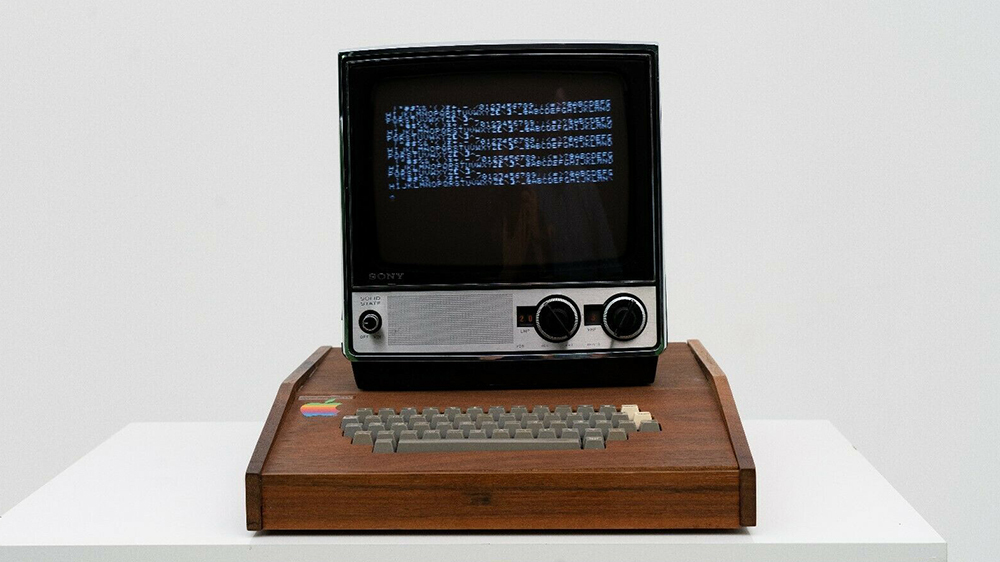
\includegraphics[width=0.4\textwidth]{apple101}
    \caption{Apples första dator: Apple 1}
    \label{fig:mesh1}
\end{figure}

Den första Appledatorn hade 4 KB i primärminne. K står för kilo (prefixet för tusen) stora b:et står för enheten byte. Är det ett litet b så är det enheten bits. Det är alltså skillnad på 1 Mb och 1 MB. Den första är 1 mega bit och den andra är 1 mega byte - alltså 8 gånger större.  

\section{Prefix och enhet}
En dator arbetar oftast med en väldigt stor mängd data. Till exempel kan en vanlig SSD-hårddisk lagra 240 gigabyte data. Det är 240 000 000 000 bytes. Men om vi ska skriva ut dessa tal hela tiden blir det snabbt jobbigt. Det är betydligt enklare att arbeta med prefix. I detta fall är giga vårt prefix. Det står för miljard. 1 gig är en miljard. Men en gig av vad? Det är där enhet kommer in. I en dator arbetar vi med enheterna bits, bytes och hertz. För att kunna avgöra hur bra något är i ett datorsystem behöver vi alltså både prefixet (hur stort/snabbt det är) och enheten. 

Det vanligaste prefixen i ett datorsystem är kilo, mega, giga och tera.\\
Kilo - 1000\\
Mega - 1 000 000\\
Giga - 1 000 000 000\\
Tera - 1 000 000 000 000\\\\\\

När använder man bits och när använder man bytes? En grundregel brukar vara att när vi pratar om hur snabbt vi kan förflytta data, till exempel genom en buss eller nätverkskabel, så används bitar. När vi pratar om data som ska lagras i till exempelt ett primärminne eller hårddisk så brukar man använda bytes. 

\chapter{Processor}
En processor brukar lite slarvigt kallas för datorns hjärna. Processorn kallas i bland för CPU vilket är en förkortning för engelskans central processing unit. Hastigheten på en processor mäts i Hertz. Hertz är antalet gånger pulsklockan i processorn under en sekund. Varje gång denna klocka slår gör processorn något. 

\section{Klockningsfrekvens}
För att ett datorsystem ska kunna göra något behöver processorns klocka skicka en puls. 
När en sån puls skickas brukar man säga att processorns pulsklocka slår. Denna klockningsfrekvens mäts i hertz. 1 Hz är ett klockslag per sekund. Eftersom en dator gör väldigt många operationer och ska göra dessa snabbt mäts oftast en processorklocka med prefixen mega eller giga. Varje gång gång klockan slår så utför processorn något. Det kan var allt ifrån att addera två tal till att flytta ett tal till från ett register till att annat. Eftersom processorn utför väldigt enkla processer stegvis krävs det oftast ett antal klockslag för att faktiskt utföra. För att till exempel addera två tal ska den först hämta båda talen från ett register (två klockslag), addera dessa två tal (ännu ett klockslag) och sedan spara resultatet i något register (ännu ett klockslag). Lägg därtil att dessa tal troligtvis har hämtats från primärminnet för att sedan lagras i processorns olika cacheminnen innan det har flyttat till processorns register. Som sagt, det krävs många klockslag för att uföra saker.\\\\
Historiskt sett har man inom processorn alltid försökt öka hertzen för att därmed få en snabbare processor. För runt tio år sen stötte man dock på ett problem. Vid runt 3,5 GHz började vi problem med värmen. Skulle vi alltså få upp klockningsfrekvens ännu mer skulle vi behöva arbeta mer med kylning. Det var då man uppfann cores. 


\end{document}
